\documentclass[conference]{IEEEtran}
\usepackage{savesym}
\usepackage{amsmath,amssymb,amsfonts,amsthm}
\usepackage[numbers]{natbib}
\usepackage{algorithm}
\usepackage[noend]{algpseudocode}
\usepackage{comment}
\usepackage{xspace}
\usepackage{scalerel}
\usepackage{xcolor}
%\usepackage[caption=false,font=footnotesize]{subfig}
\usepackage[left]{showlabels}
\usepackage{multicol}
\usepackage[bookmarks=true]{hyperref}
\usepackage{graphicx,subfigure}

\begin{document}

\title{	Online, interactive user guidance for \\
		high-dimensional, constrained motion planning }

\author{Fahad Islam, Oren Salzman and Maxim Likhachev}


\maketitle
\thispagestyle{empty}
\pagestyle{empty}

\def\frechet{Fr\'echet\xspace}

\newcommand{\cupdot}{\mathbin{\mathaccent\cdot\cup}}

%unlabeled PSPACE-hardness paper
\newcommand{\mtm}{\emph{multi-to-multi}\xspace}
\newcommand{\mts}{\emph{multi-to-single}\xspace}
\newcommand{\sts}{\emph{multi-to-single-restricted}\xspace}
\newcommand{\dtd}{\emph{single-to-single}\xspace}

\newcommand{\cte}{\emph{full-to-edge}\xspace}
\newcommand{\ctc}{\emph{full-to-full}\xspace}
\newcommand{\ete}{\emph{edge-to-edge}\xspace}

\newcommand{\AND}{{\sc and}\xspace}
\newcommand{\OR}{{\sc or}\xspace}

%tex tools
\newcommand{\ignore}[1]{}

%%% algorithms
\def\vor{\text{Vor}}

\def\P{\mathcal{P}} \def\C{\mathcal{C}} \def\H{\mathcal{H}}
\def\F{\mathcal{F}} \def\U{\mathcal{U}} \def\L{\mathcal{L}}
\def\O{\mathcal{O}} \def\I{\mathcal{I}} \def\E{\mathcal{E}}
\def\S{\mathcal{S}} \def\G{\mathcal{G}} \def\Q{\mathcal{Q}}
\def\I{\mathcal{I}} \def\T{\mathcal{T}} \def\L{\mathcal{L}}
\def\N{\mathcal{N}} \def\V{\mathcal{V}} \def\B{\mathcal{B}}
\def\D{\mathcal{D}} \def\W{\mathcal{W}} \def\R{\mathcal{R}}
\def\M{\mathcal{M}} \def\X{\mathcal{X}} \def\A{\mathcal{A}}
\def\Y{\mathcal{Y}} \def\L{\mathcal{L}}

\def\dS{\mathbb{S}} \def\dT{\mathbb{T}} \def\dC{\mathbb{C}}
\def\dG{\mathbb{G}} \def\dD{\mathbb{D}} \def\dV{\mathbb{V}}
\def\dH{\mathbb{H}} \def\dN{\mathbb{N}} \def\dE{\mathbb{E}}
\def\dR{\mathbb{R}} \def\dM{\mathbb{M}} \def\dm{\mathbb{m}}
\def\dB{\mathbb{B}} \def\dI{\mathbb{I}} \def\dM{\mathbb{M}}

\def\eps{\varepsilon}
\def\obs{\mathrm{obs}}

\newcommand{\sbs}{sampling-based\xspace}
\newcommand{\mr}{multi-robot\xspace}
\newcommand{\mpl}{motion planning\xspace}
\newcommand{\cs}{configuration space\xspace}
\newcommand{\conf}{configuration\xspace}
\newcommand{\confs}{configurations\xspace}
\newcommand{\etal}{et al.\xspace}

% programming
\newcommand{\Cpp}{C\raise.08ex\hbox{\tt ++}\xspace}



\newcommand{\ch}{\mathrm{ch}}
\newcommand{\pspace}{{\sc pspace}\xspace}
\newcommand{\np}{{\sc np}\xspace}
\newcommand{\degree}{\ensuremath{^\circ}}
\newcommand{\argmin}{\operatornamewithlimits{argmin}}


\newcommand{\dist}{\textup{dist}}

\newcommand{\Cfree}{\C_{\textup{free}}}
\newcommand{\Cforb}{\C_{\textup{forb}}}

\newtheorem{lemma}{Lemma}
\newtheorem{theorem}{Theorem}
\newtheorem{corollary}{Corollary}
\newtheorem{claim}{Claim}

\newtheorem{definition}{Definition}
\newtheorem{remark}{Remark}
\newtheorem{observation}{Observation}

\def\os#1{\textcolor{blue}{#1}}
\def\ToDo#1{\textcolor{magenta}{\textbf{ToDo:}~#1}}


\makeatletter
\def\thmhead@plain#1#2#3{%
  \thmname{#1}\thmnumber{\@ifnotempty{#1}{ }\@upn{#2}}%
  \thmnote{ {\the\thm@notefont#3}}}
\let\thmhead\thmhead@plain
\makeatother

\def\todo#1{\textcolor{blue}{\textbf{TODO:} #1}}
\def\new#1{\textcolor{magenta}{#1}}
\def\old#1{\textcolor{red}{#1}}

\def\removed#1{\textcolor{green}{#1}}
%\def\removed#1{}
%%% Local Variables:
%%% mode: plain-tex
%%% TeX-master: "main"
%%% End:
\algrenewcommand\textproc{}

\newcommand\algname[1]{\textsf{#1}\xspace}
\newcommand\astar{\algname{A*}}
\newcommand\mhastar{\algname{MHA*}}

\newcommand{\arxiv}[2]{#1}

\begin{abstract}
We consider the problem of planning a collision-free path for a high-dimensional robot.
Specifically, we suggest a planning framework where a motion-planning algorithm can obtain guidance from a user.
In contrast to existing approaches, we suggest to seek user guidance only when the planner identifies that it ceases to make significant progress towards the goal.
User guidance is given in the form of an intermediate configuration~$\hat{q}$ which, in turn, is used to bias the planner to go through $\hat{q}$.
We demonstrate our approach for the case where the planning algorithm is Multi-Heuristic A* (MHA*) and the robot is a 34-DOF humanoid.
We show that using this general approach allows to compute highly-constrained paths such as climbing stairs with little domain knowledge.
Without our approach, solving such problems require carefully-crafted domain-dependant  heuristics. 
\end{abstract}

\IEEEpeerreviewmaketitle

%%%%%%%%%%%%%%%%%%%%%%%%%%%%%%%%%%%%%%%%%%%%%%%%%%%%%
%Intro
%%%%%%%%%%%%%%%%%%%%%%%%%%%%%%%%%%%%%%%%%%%%%%%%%%%%%
%\begin{comment}
\section{Introduction}
\label{sec:intro}

Motion-planning is a fundamental problem in robotics that has been studied for over four decades~\cite{CBHKKLT05,L06,S04}.
However, efficiently planning paths in high-dimensional, constrained spaces remains an ongoing challenge.
One approach to address this challenge is to incorporate user input to guide the motion-planning algorithm.
While there has been much work on planning using human demonstration 
(see, e.g.,~\cite{ACVB09, HS16, PHCL16, SHLA16, YA17}), 
there has been far less research incorporating guidance as an interactive part of the planning~loop.

Broadly speaking, interactive planning has been typically used in the context of sampling-based motion-planning algorithms~\cite{L06}.
User guidance was employed by biasing the sampling scheme of the planner.
This was done by having the user mark regions in the \emph{workspace} that should be avoided or 
%explored~\cite{DSJA14}.
explored~\cite{DSJA14, MTMKDC15, YPB15}.
%\os{Mention Vinitha's paper when arXived}
Alternatively, interactive devices such as a 3D mouse or a haptic arm have been used to generate paths in a (low-dimensional) configuration space. This path was then used by a planner to bias its 
%sampling domain~\cite{TFF12}.
sampling domain~\cite{BTFF16, FTF09, TFF12}.
%Interestingly, in all the examples mentioned, an implicit assumption taken is that the user is dedicated to guide and interact with the planning algorithm.

We are interested in planning in high-dimensional, constrained spaces such as those encountered by a humanoid robot (see Fig.~\ref{fig:robot} and Sec.~\ref{sec:rel}).
In such settings, workspace regions often give little guidance to the planner due to the high dimension of the configuration space as well as the physical constraints of the robot.
Additionally, obtaining user guidance in the configuration space is extremely time consuming, even for expert users.
Thus,  while beneficial, user guidance should be employed scarcely.

Our key insight is that carefully chosen individual configurations suggested by a user can be used to effectively guide the planner when in need.
Transforming this insight into a planning framework requires addressing three fundamental questions:

\begin{itemize}
	\item[\textbf{Q1.}] When should the planner ask the user for guidance?
	\item[\textbf{Q2.}] What form should the user's guidance take?
	\item[\textbf{Q3.}] How should the guidance be used by the planner?
\end{itemize}

Identifying \emph{when} to obtain guidance 
(Q1, Sec~\ref{sec:q1}) 
comes in stark contrast to existing approaches---we suggest to only employ user guidance when the planner \emph{identifies} that it ceases to make significant progress towards the goal.
The specific type of guidance given 
(Q2, Sec~\ref{sec:q2}),
as previously mentioned,
is configuration-space based and \emph{not} workspace-based. This deviation from previous work is due to our specific setting of high-dimensional, constrained systems.
Finally, guidance is used to \emph{bias} the search algorithm towards regions that are likely to be beneficial (Q3, Sec~\ref{sec:q2}). 
It is worth emphasising that this is done without requiring the user to understand the underlying search algorithm. 

% 
%In the following, we detail our planning framework (Sec.~\ref{sec:high}) and how it addresses each of these questions (Sec.~\ref{sec:q1}-\ref{sec:q3}).
%We then continue (Sec.~\ref{sec:eval}) to demonstrate its effectiveness in simulations and conclude by describing possible additional future work.

\begin{figure}[tb]
  \centering
  	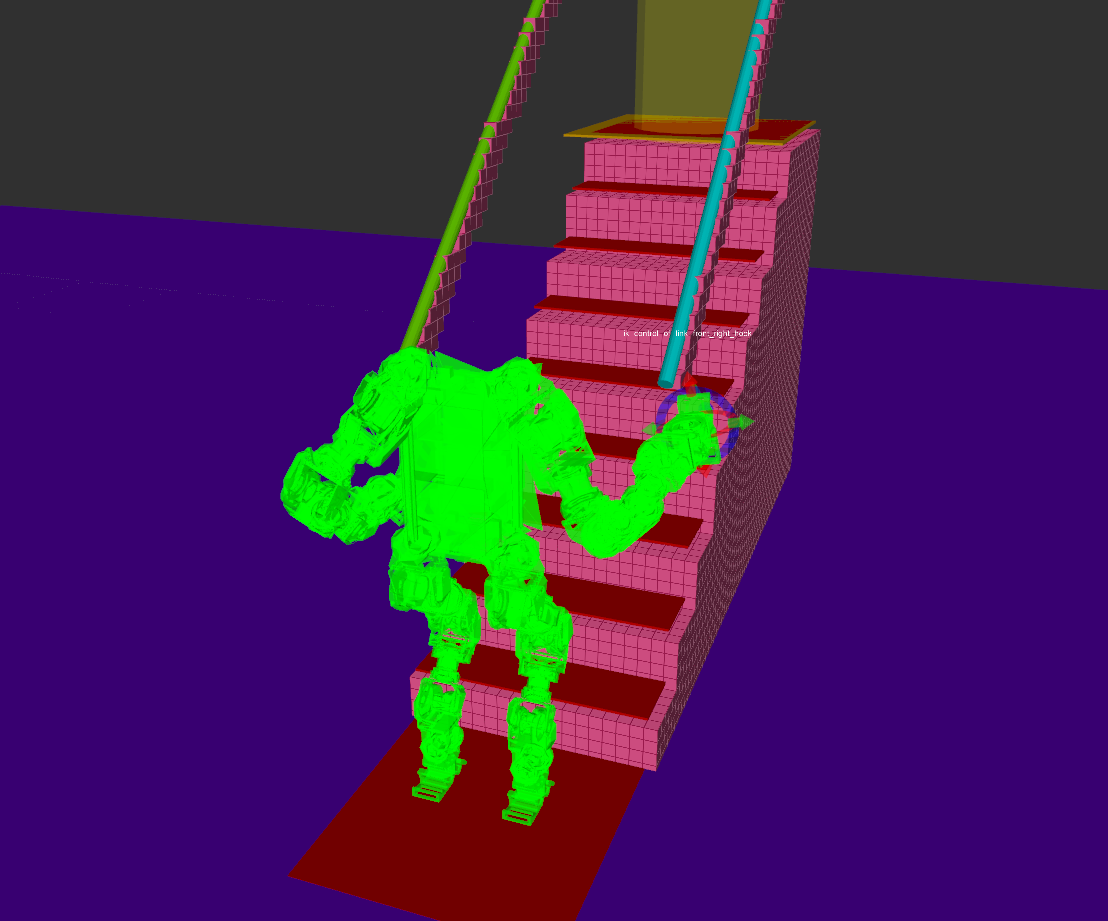
\includegraphics[width=0.283\textwidth]{fig/workspace.png}
  	%\vspace{-2mm}
  \caption{
		Planning domain---Humanoid robot needs to climb the stairs while avoiding collision with the obstacles and while adhering to the physical stability constraints.
  	\vspace{-15mm}
}
   	\label{fig:robot}
\end{figure}



%\section{Related work}
%\label{sec:related}
%

While our approach is general and can be incorporated with any motion-planning algorithm (see discussion in Sec.~\ref{sec:future}) it is especially suitable for search-based planning algorithms (see, e.g.,~\cite{CCL14}) that perform a systematic search guided by heuristic functions.
Specifically, we demonstrate it's effectiveness for the case where the motion-planning algorithm is multi-heuristic A* (MHA*)~\cite{ASNHL16, NAL15} which we detail in Sec.~\ref{sec:mha}.
%MHA* is a search-based planning algorithm that takes in multiple, possibly inadmissible heuristic functions in addition to a single consistent admissible heuristic.
%It uses them simultaneously to search the configuration space in an A*-like manner that was shown to be both complete and ensures bounds on sub-optimality. 
%This allows the search to efficiently combine the guiding powers of different heuristic functions. 




After describing our approach at high-level (Sec.~\ref{sec:high}) we demonstrate how it can be applied to the case of MHA* (Sec.~\ref{sec:planning}).
We continue by showing the effectiveness of our planner (Sec.~\ref{sec:eval}).
Specifically, we show that this general approach allows to compute highly-constrained paths such as climbing stairs with little domain knowledge.
Without our approach, solving such problems require carefully-crafted domain-dependant heuristics. 
We conclude this paper with a discussion and an outline of possible future work (Sec.~\ref{sec:future}).


\section{Related work and algorithmic background}
\subsection{Motion planning for humanoid robots}
\label{sec:rel}
Humanoid robots, for which we demonstrate our approach, often have several dozens of degrees of freedom making planning a challenging task, especially when taking additional constraints into account such as stability and contact constraints.
One approach to plan the motion for such systems, is to use predefined, carefully chosen fixed gaits~\cite{KKKHKHAI04}. 
However, when the terrain is uneven, such planners are inadequate at computing stable motions~\cite{HBLHW08}.
Another approach is to reduce the search space by decomposing the degrees of freedom into functional groups such as locomotion and manipulation.
Then functional-specific algorithms such as footstep planning are applied to the low-dimensional space (see, e.g.,~\cite{CLCKHK05, KNKII01, PSBLY12, XCXZC09, KKNII02} for a prtial list).
A high-dimensional planner is then used to ``track'' the plan generated in the low-dimensional space.

In this work, we employ the recently-introduced adaptive dimensionality framework~\cite{GCBSL11, GSL12, GSL13}.
Roughly speaking,  it consists of two stages: an adaptive planning phase which attempts to plan in a low-dimensional space when possible and a tracking phase which plans in the high-dimensional space.
Our user-guided planner is integrated within the high-dimensional planner.

\subsection{Multi Heuristic A* (MHA*)}
\label{sec:mha}
Multi Heuristic A* (MHA*)~\cite{ASNHL16, NAL15} is a search-based planning algorithm that takes in multiple, possibly inadmissible heuristic functions in addition to a single consistent admissible heuristic termed the \emph{anchor} heuristic.
It then uses the heuristic functions to simultaneously perform a set of A*-like searches.
Using multiple searches allows the algorithm to efficiently combine the guiding powers of the different heuristic functions. 

Specifically, for each search, MHA* uses a separate priority queues associated with each heuristic. 
The algorithm iterates between the searches in a structured manner that ensures bounds on sub-optimality. 
This can be done in a round-robin fashion, or using more 
sophisticated approaches that allow to automatically calibrate the weight given to each heuristic~\cite{PNAL15}.

Part of the efficiency of MHA* is due to the fact that the value of the cost-to-come (the $g$-value) computed for each state is shared between all the different searches\footnote{To be precise, Aine et al.~\cite{ASNHL16} define two variants of MHA*: Independent and Shared MHA* where the queues do not share and do share the $g$-values of states, respectively. In this paper when we use the term MHA* to refer to the latter (shared) variant.}.
Sharing cost-to-come values between searches implies that if a better path to a state is discovered by any of the searches, the information is updated in all the
priority queues. 
Moreover, if one search ceases to make progress towards the goal (a state which we call ``stagnation region'' and which will be formally defined in Sec.~\ref{sec:planning}) it can use ``promising'' states found by other searches to escape this stagnation region (see also~\cite{HB12, I92}).
Furthermore, path sharing allows SMHA* to expand each state at most twice.
Finally, using heuristics gives a principled way to identify when the planner ceases to make progress (see, e.g.,~\cite{VNL17}).


%heuristic depression
%regions, i.e., regions in the search space where the correlation between the heuristic values and the actual cost-to-go is
%weak
%
%Intuitively, a heuristic depression is a bounded region of the search space
%in which the heuristic is inaccurate with respect to the heuristic values of the states in
%the border of the region
%
%Ishida (1992) gave a constructive definition for \textbf{heuristic depressions}. The construction
%starts with a node s such that its heuristic value is equal to or less than those of the
%surrounding states. The region is then extended by adding a state of its border if all states
%in the resulting region have a heuristic value lower or equal than those of the states in the
%border. As a result, the heuristic depression D is a maximal connected component of states
%such that all states in the boundary of D h




\section{Algorithmic approach---user-guided planning}
\label{sec:high}

\algrenewcommand\algorithmicindent{.8em}
\begin{algorithm}[tb]
\caption{User-guided planning ($\A$)}
\label{alg:main}	
\begin{algorithmic}[1]
\small
\While{$\neg\A.$\texttt{is\_solution\_found()} } 
	\While{$\neg\A.$\texttt{is\_in\_stagnation\_region()}} 
		\State $\A.$\texttt{run()}
		\Comment{no user guidance}
	\EndWhile
%	
	\State {$g \leftarrow$ \texttt{get\_user\_guidance()}}
	\Comment{$\A$ is in a stagnation region}
	\State $\A.$\texttt{update\_user\_guidance($g$)}
	\Comment{account for guidance}
	\While{$\A.$\texttt{is\_in\_stagnation\_region()}}
		\State $\A.$\texttt{run()}
		\Comment{$\A$ uses guidance to escape stagnation region}
	\EndWhile

	\State $\A.$\texttt{update\_user\_guidance($\neg g$)}
	\Comment {remove  guidance}
\EndWhile
\end{algorithmic}
\end{algorithm}

To employ our planning framework, we assume that we are given a motion-planning algorithm $\A$ that is endowed with two non-standard procedures which are planner dependent.
The first, \texttt{is\_in\_stagnation\_region()}, 
identifies when it is in a \emph{stagnation region}, namely when $\A$'s search does not progress towards the goal. 
The second, \texttt{update\_user\_guidance()}, 
incorporates (or removes) the user guidance provided to $\A$. 

Equipped with these functions, we can describe our planning framework, detailed in Alg.~\ref{alg:main}.
The framework runs as long as no solution is found (line~1).
It runs the planner~$\A$ (lines~2-3) as long as it continuously makes progress towards the goal (namely, it is not in a stagnation region).
Once a stagnation region is identified, user guidance is invoked (line~4) and $\A$  is updated to make use of this guidance (line~5).
It is then run while using the guidance as long as it is still in the stagnation region (lines~6-7).
Once it escapes the stagnation region $\A$ is updated to remove the guidance that was provided by the user (line~8).


\section{User-guided planning via MHA*}
\label{sec:planning}

We demonstrate our general planning framework described in Sec.~\ref{sec:high} for the case where the motion-planning algorithm~$\A$ is multi-heuristic A* (MHA*)~\cite{ASNHL16}.
We assume that MHA* has a set of \emph{baseline heuristics} (the anchor heuristic and possibly additional heuristics).
The user guidance will be used to generate \emph{dynamic heuristics}.
We start (Sec.~\ref{sec:q1}-\ref{sec:q3}) by describing how we answer the three questions we posed in Sec.~\ref{sec:intro}.
We then continue to detail how they are used in our planning framework.
This implementation is slightly more complicated than that described in Alg.~\ref{alg:main} and is detailed in Sec.~\ref{sec:instantiation}.

\subsection{Invoking user guidance (Q1)}
\label{sec:q1}


\begin{figure*}[t]%
%\captionsetup{format = plain}
  \centering%
  \subfigure[]
  {
  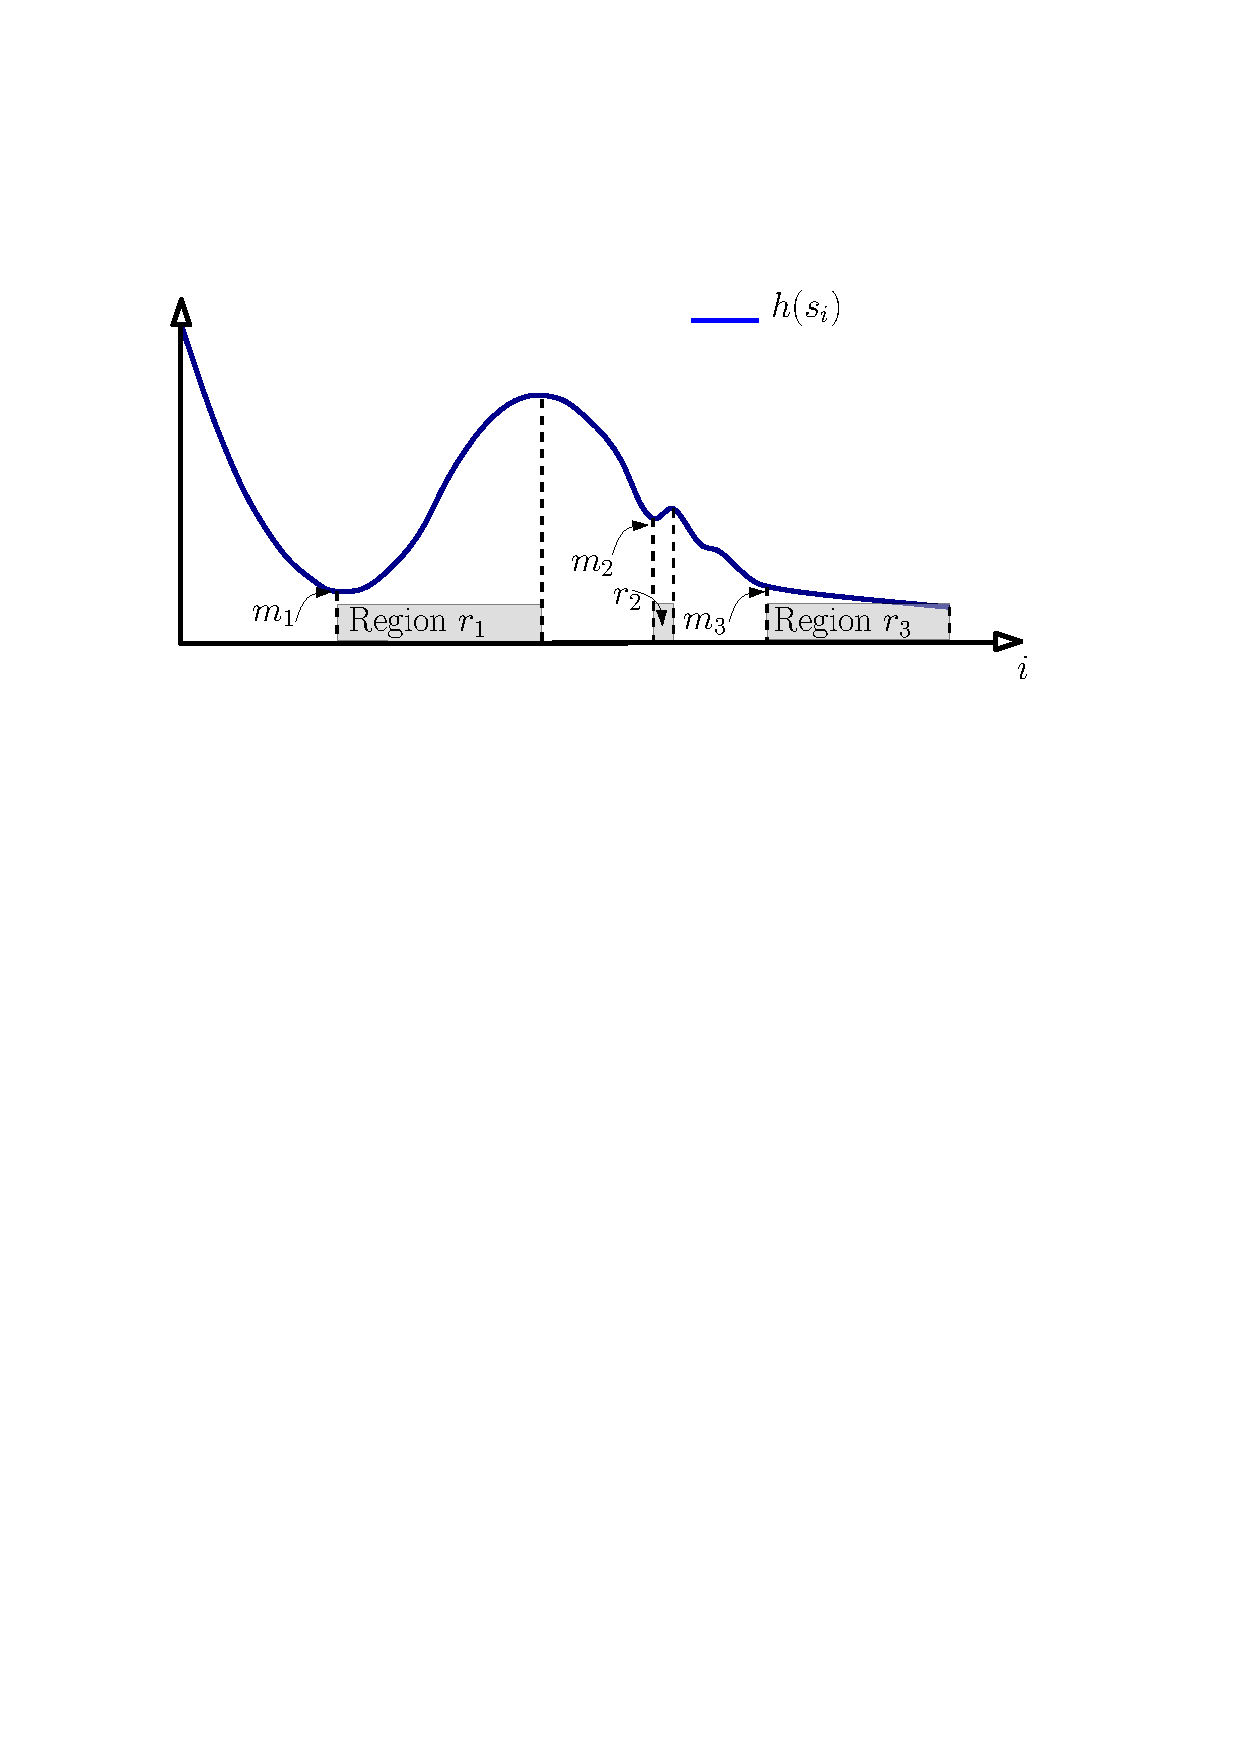
\includegraphics[width=0.34\textwidth]{fig/local_min_detection_1.pdf}
  \label{fig:local_min1}
  }
  \hspace{-10mm}
%  \subfigure[]
%  {
%  \label{fig:local_min2}
%  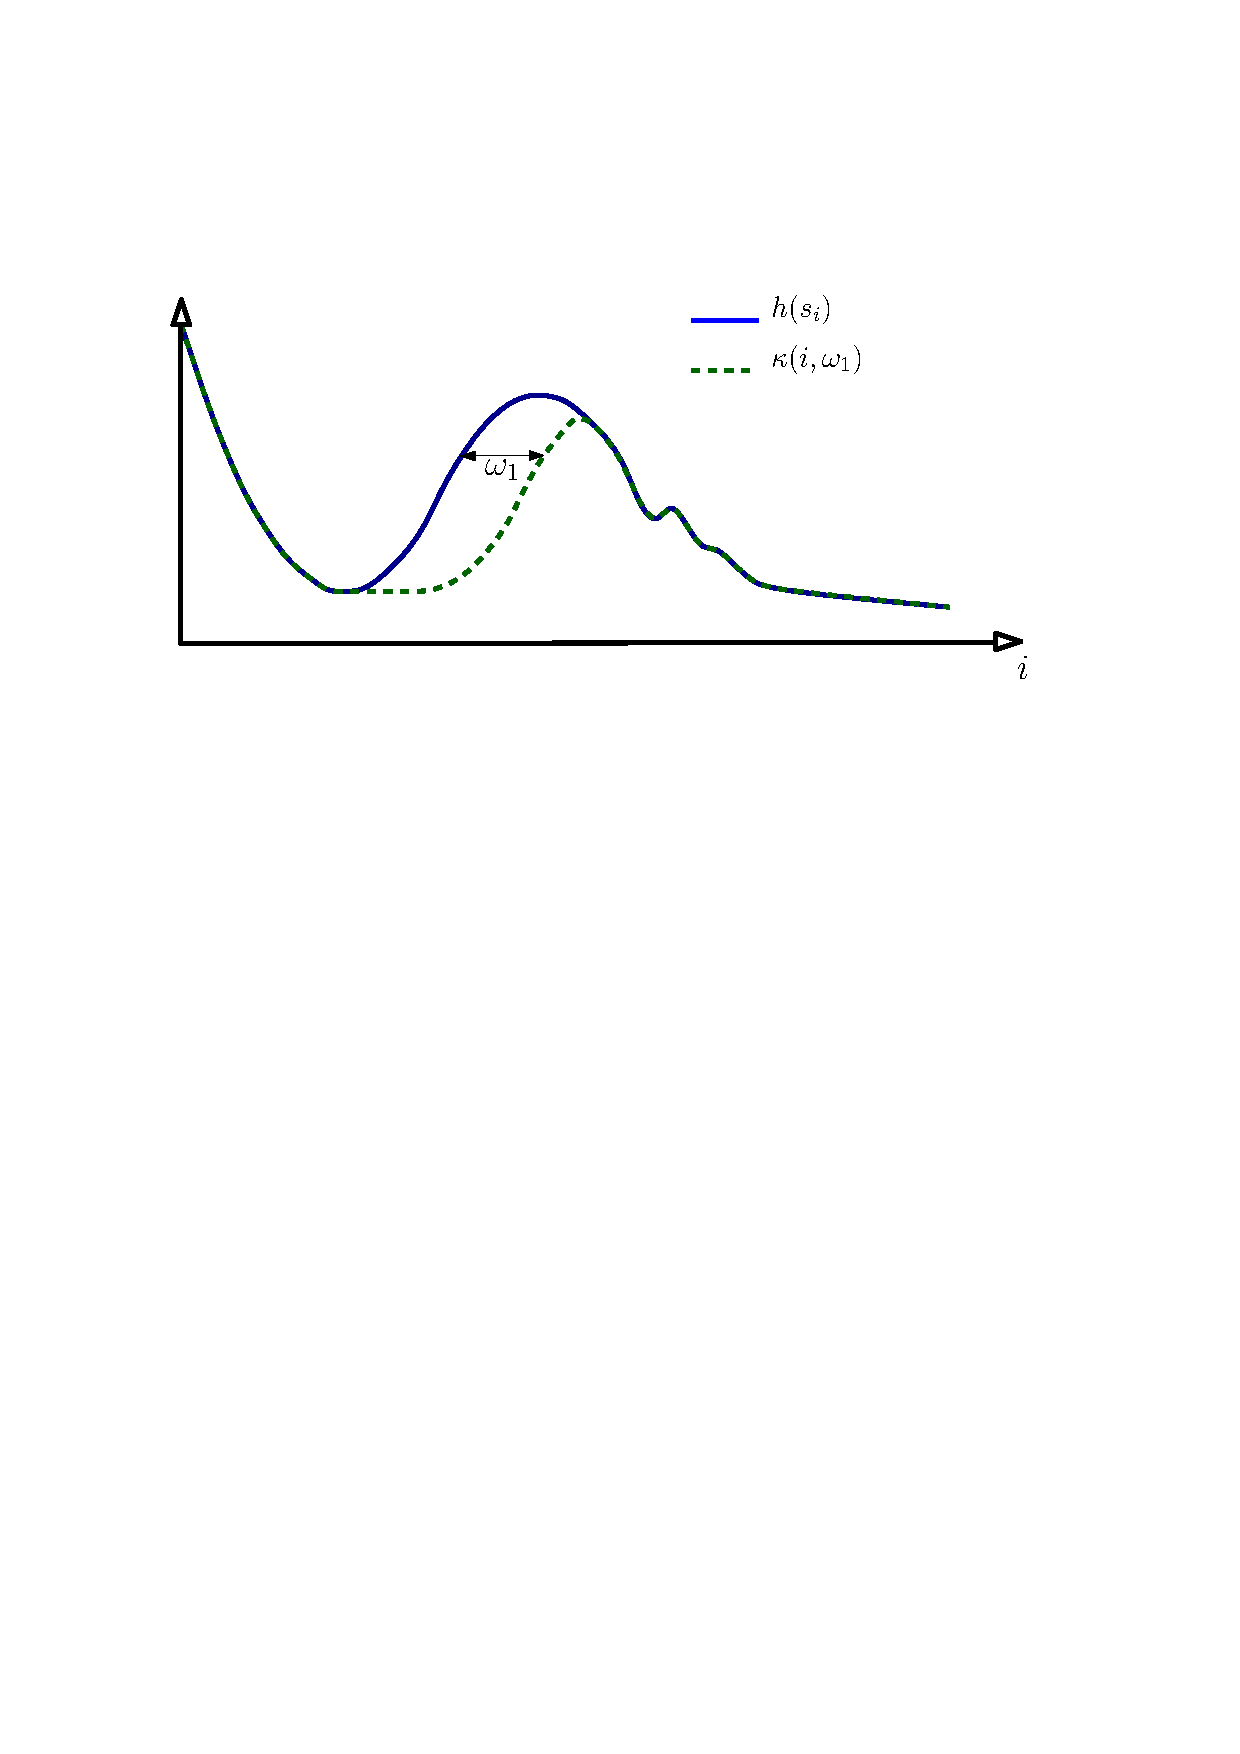
\includegraphics[width=0.265\textwidth]{fig/local_min_detection_2.pdf}
%  }
%  \hspace{-10mm}
  \subfigure[]
  {
  \label{fig:local_min3}
  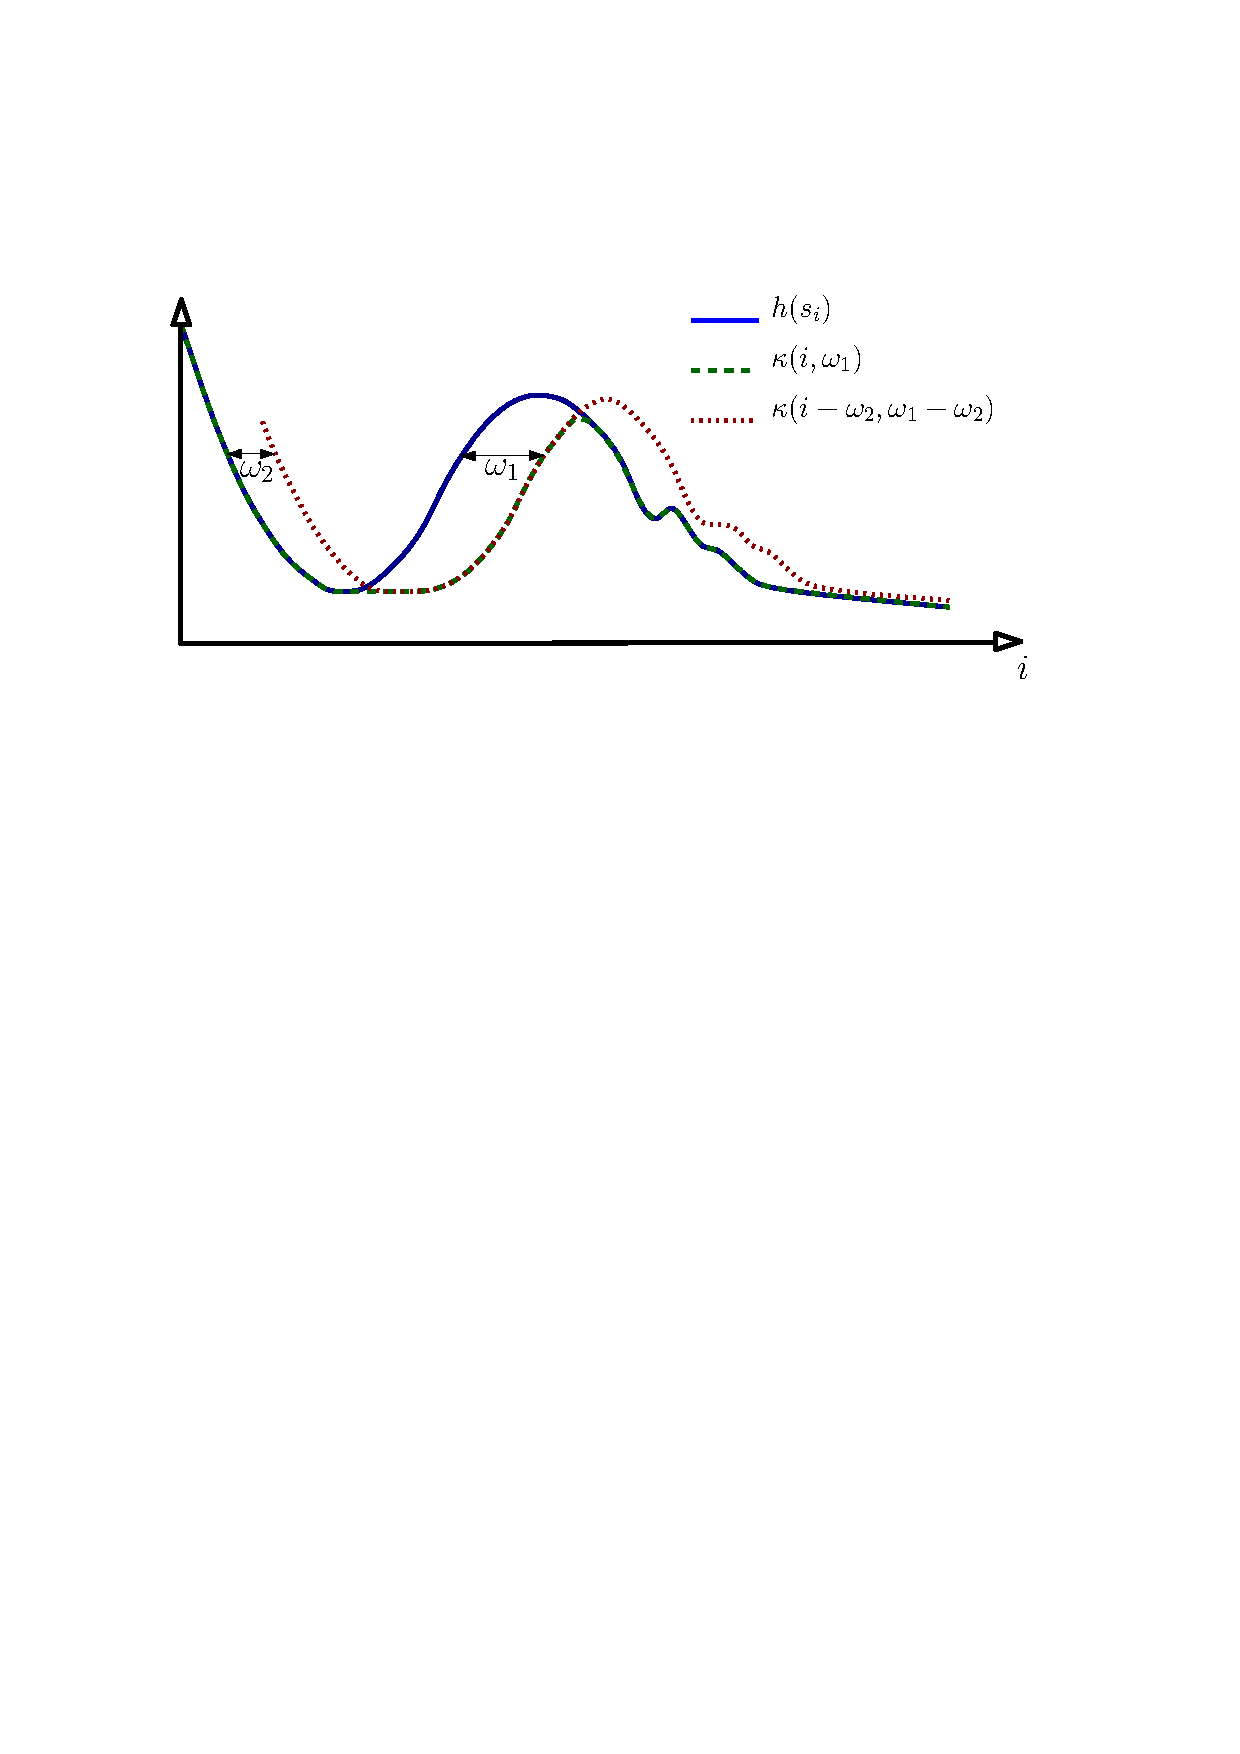
\includegraphics[width=0.34\textwidth]{fig/local_min_detection_3.pdf}
  }  
  \hspace{-10mm}
  \subfigure[]
  {
  \label{fig:local_min4}
  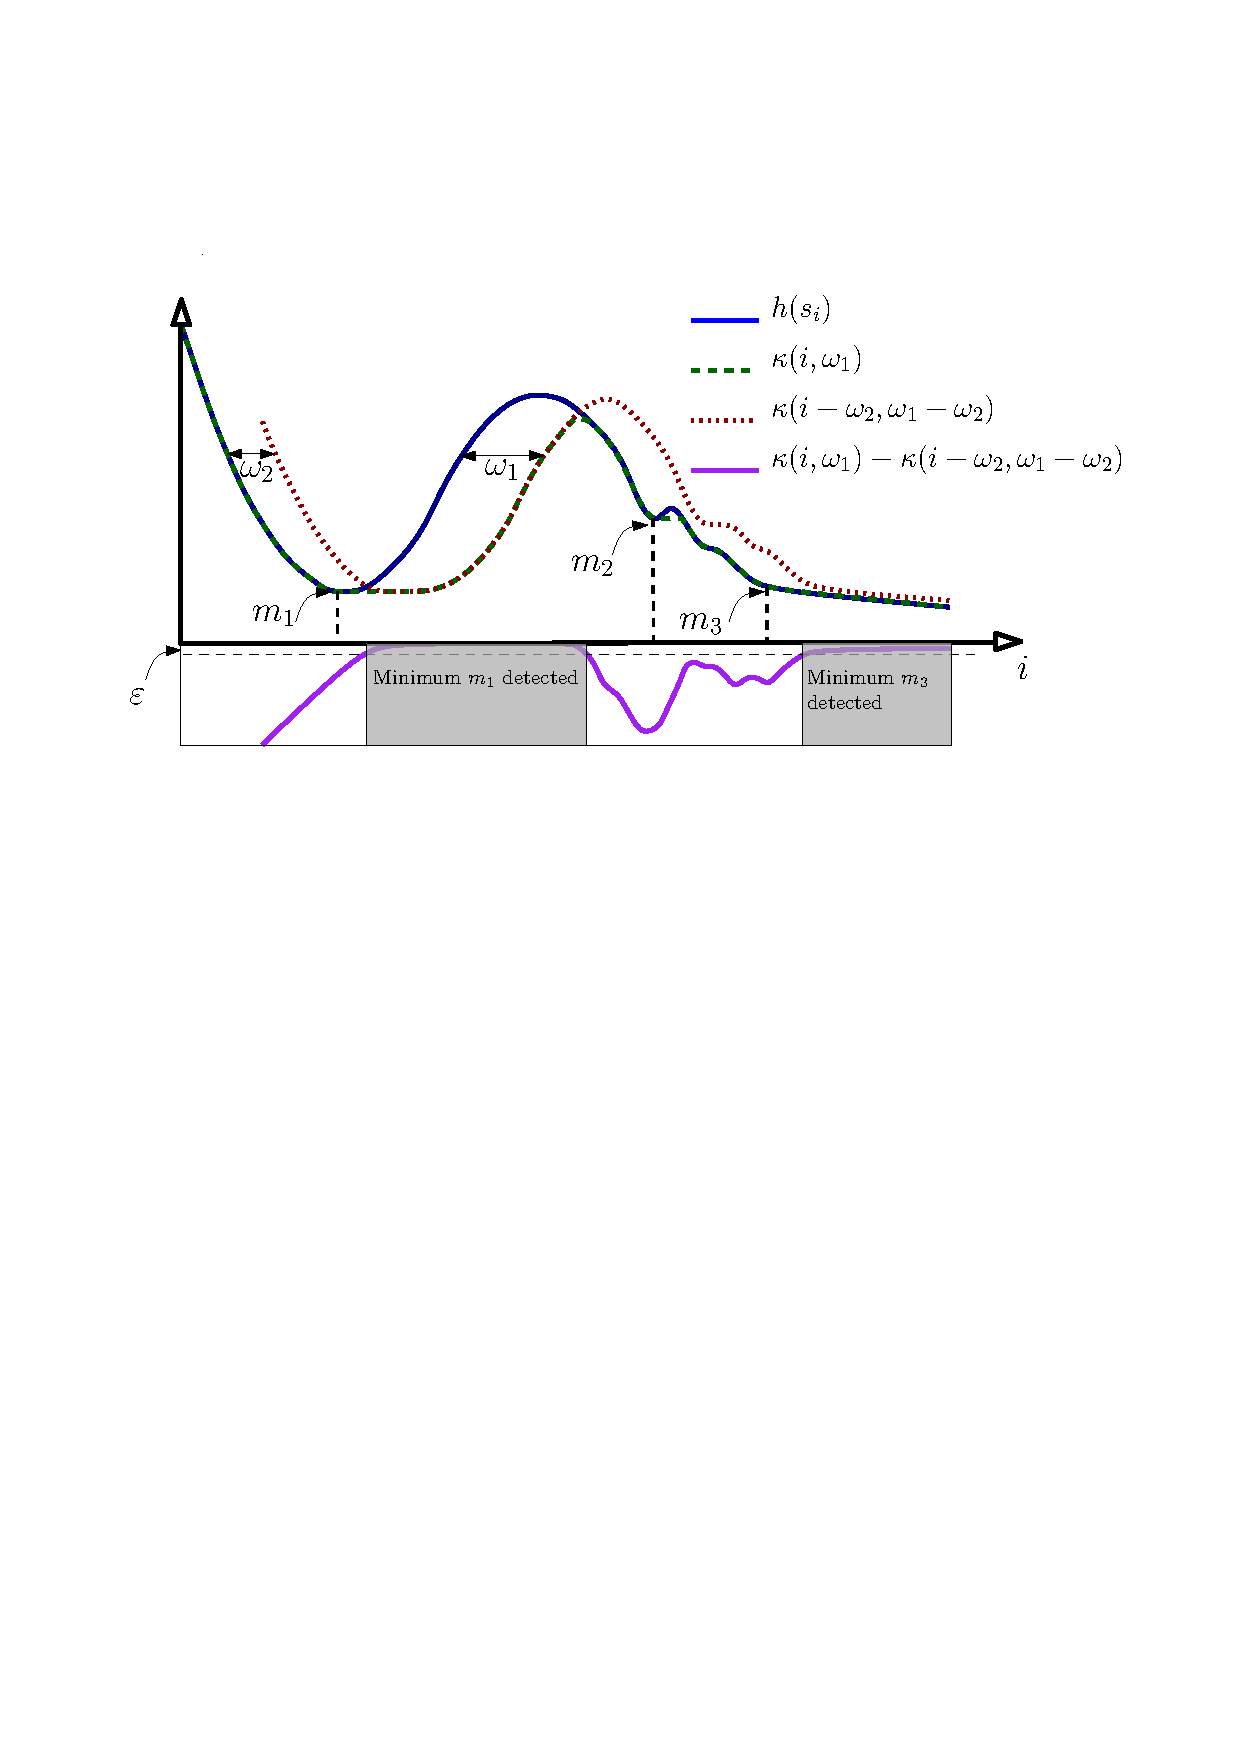
\includegraphics[width=0.34\textwidth]{fig/local_min_detection_4.pdf}
  }
  \vspace{-1mm}
  \caption{%
    Visualization of the way stagnation regions are detected.   
	\subref{fig:local_min1}~The heuristic value $h(s_i)$ (solid blue) has three local minima, $m_1, m_2$ and $m_3$ followed by three stagnation regions (light grey). Local minima $m_2$ is very small while~$m_3$ is not a local minimum per se, yet the progress made between consecutive steps is smaller than the predefined threshold~$\varepsilon$.
    %
    \subref{fig:local_min3}~The function $\kappa(i,\omega_1)$ (dashed green) returns the minimal value $h(s_i)$ attained over the past~$\omega_1$ iterations (referred to  as the ``recent history'').
    %
%    \subref{fig:local_min3}~
    The function $\kappa(i-\omega_2,\omega_1-\omega_2)$ (dotted red) returns the minimal value $h(s_i)$ attained over the beginning of the recent history.
    %
    \subref{fig:local_min4}~The difference between the two functions (solid purple) indicates if there was significant progress (i.e. more than $\varepsilon$) made at the end of the recent horizon when compared to the beginning of the recent history. 
    If not, then the planner detects a stagnation region (dark grey).
		Notice that the hysteresis parameters~$\omega_1$ and $\omega_2$ 
		(i)~induce a lag from the time that the stagnation region starts until it is detected,
		(ii)~allow to avoid detecting stagnation region~$r_2$.  
		}%

  \label{fig:filmstrip-local-min}%

  \vspace{-4.5mm}

\end{figure*}


The heuristic functions of search-based planning algorithms, such as MHA*, can be used to estimate in a principled manner when the planner is in a stagnation region (Alg~\ref{alg:main}, lines 2, 6). 
%Specifically, in such algorithms,  we proceed by iteratively choosing  the current-best state from a priority queue and computing all its successors. 
%
We suggest to identify when the planner is in a stagnation region as follows:
Let~$\Q$ be a priority queue 
ordered according to some heuristic function~$h(\cdot)$,
$s_i$ be the node expanded from~$\Q$ at the $i$'th iteration and $\omega_1, \omega_2$ be parameters such that $\omega_1 > \omega_2$.
%
We define 
$\kappa_\Q(i, \omega) = \min_{i-\omega \leq j \leq i} \{ h(s_j)\}$.
Namely, $\kappa_\Q(i, \omega)$ denotes the minimal value attained by $h$ in the past~$\omega$ states. 
%
\begin{definition}
A heuristic~$h$ associated with a queue~$\Q$ is defined to be in a stagnation region if 
$\kappa_\Q(i, \omega_1) \geq \kappa_\Q(i - \omega_2, \omega_1 - \omega_2) - \varepsilon$.
\end{definition}
\noindent Namely,~$\Q$ is in a stagnation region if looking at the previous~$\omega_1$ iterations, 
there was no reduction 
(by more than some threshold $\varepsilon$) 
in the minimum value of~$h$ 
in the last $\omega_2$ states expanded from $\Q$.

%\begin{definition}
%MHA* is defined to be in a local minimum if 
%all it's queues are in local minima.
%\end{definition}

Thus, our algorithm is given three additional parameters~$\omega_1, \omega_2$ and $\varepsilon$ 
and maintains  for each queue~$\Q$ the values~$\kappa_\Q(i, \omega_1)$ and $\kappa_\Q(i - \omega_2, \omega_1 - \omega_2)$.
Note that testing if a single queue is in a stagnation region takes $O(1)$ time.
For a visualization, see Fig.~\ref{fig:filmstrip-local-min}.

\os{mention that if the heuristic is incomplete it can be defined to be in a stagnation region while the planner will  actually make progress}
\subsection{Form of user guidance (Q2)}
\label{sec:q2}
We chose to obtain user guidance 
(Alg~\ref{alg:main}, line~4)
in the form of an intermediate configuration $\hat{q}$ that is used to guide the planner. We discuss alternative options in Sec.~\ref{sec:future}.

The framework includes a graphical user interface (GUI)
\os{add pic of GUI} capable of  depicting the robot and the workspace.
Once user guidance is invoked, 
a configuration in the stagnation region is obtained and the robot is placed in that configuration (as well as the start configuration and target region) in the GUI.
This allows the user to intuitively try and understand where the planner faces difficulty and how to guide it out of the stagnation region.
The user then suggests the guidance $\hat{q}$ by moving the robot's joints and end effectors.
We note that the user is \emph{not} required to be familiar with the search algorithm.

\subsection{Using user guidance (Q3)}
\label{sec:q3}
\noindent 
\os{mention that we can add a queue for every baseline heuristic}



\begin{figure*}[t]%
%\captionsetup{format = plain}
  \centering%
  \subfigure[]
  {
  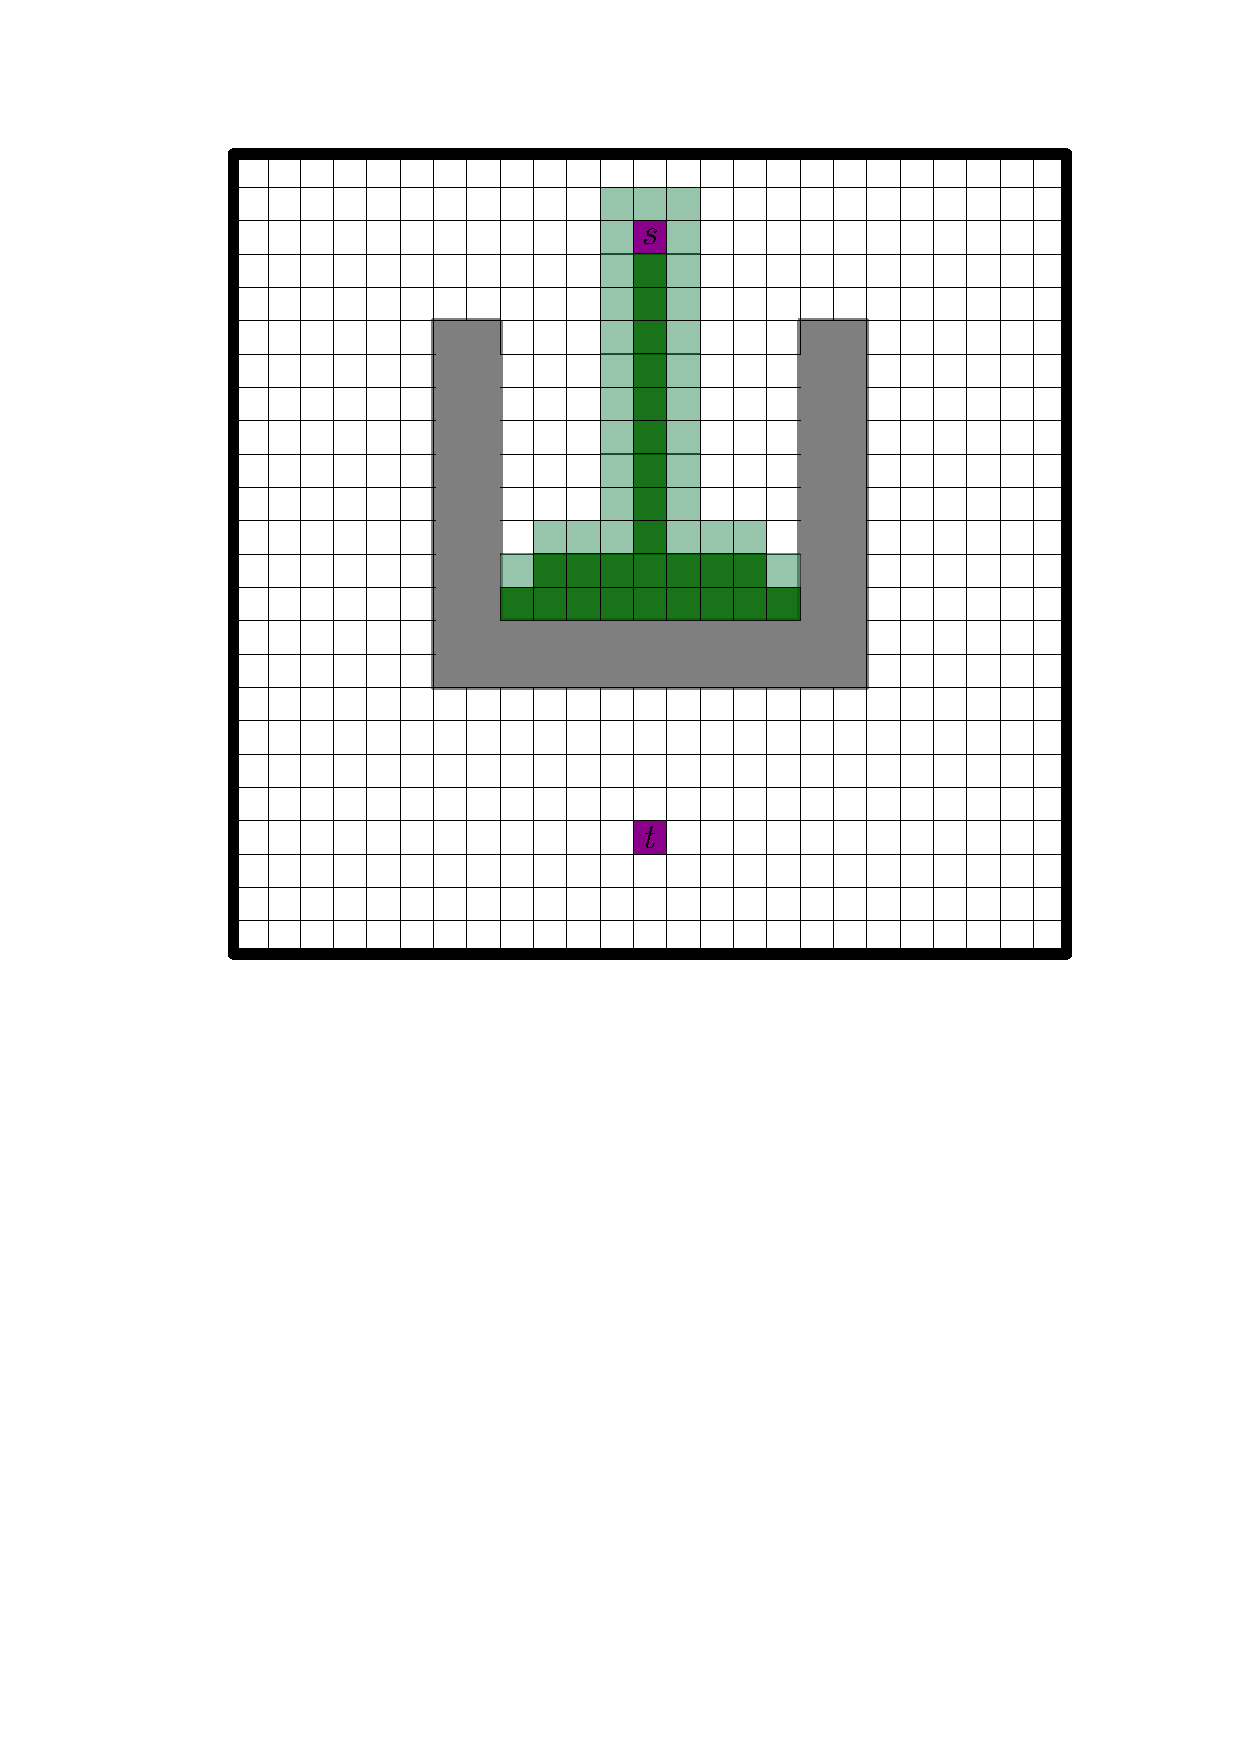
\includegraphics[width=0.225\textwidth]{fig/example_1.pdf}
  \label{fig:dynamic_heuristic1}
  }
  \subfigure[]
  {
  \label{fig:dynamic_heuristic2}
  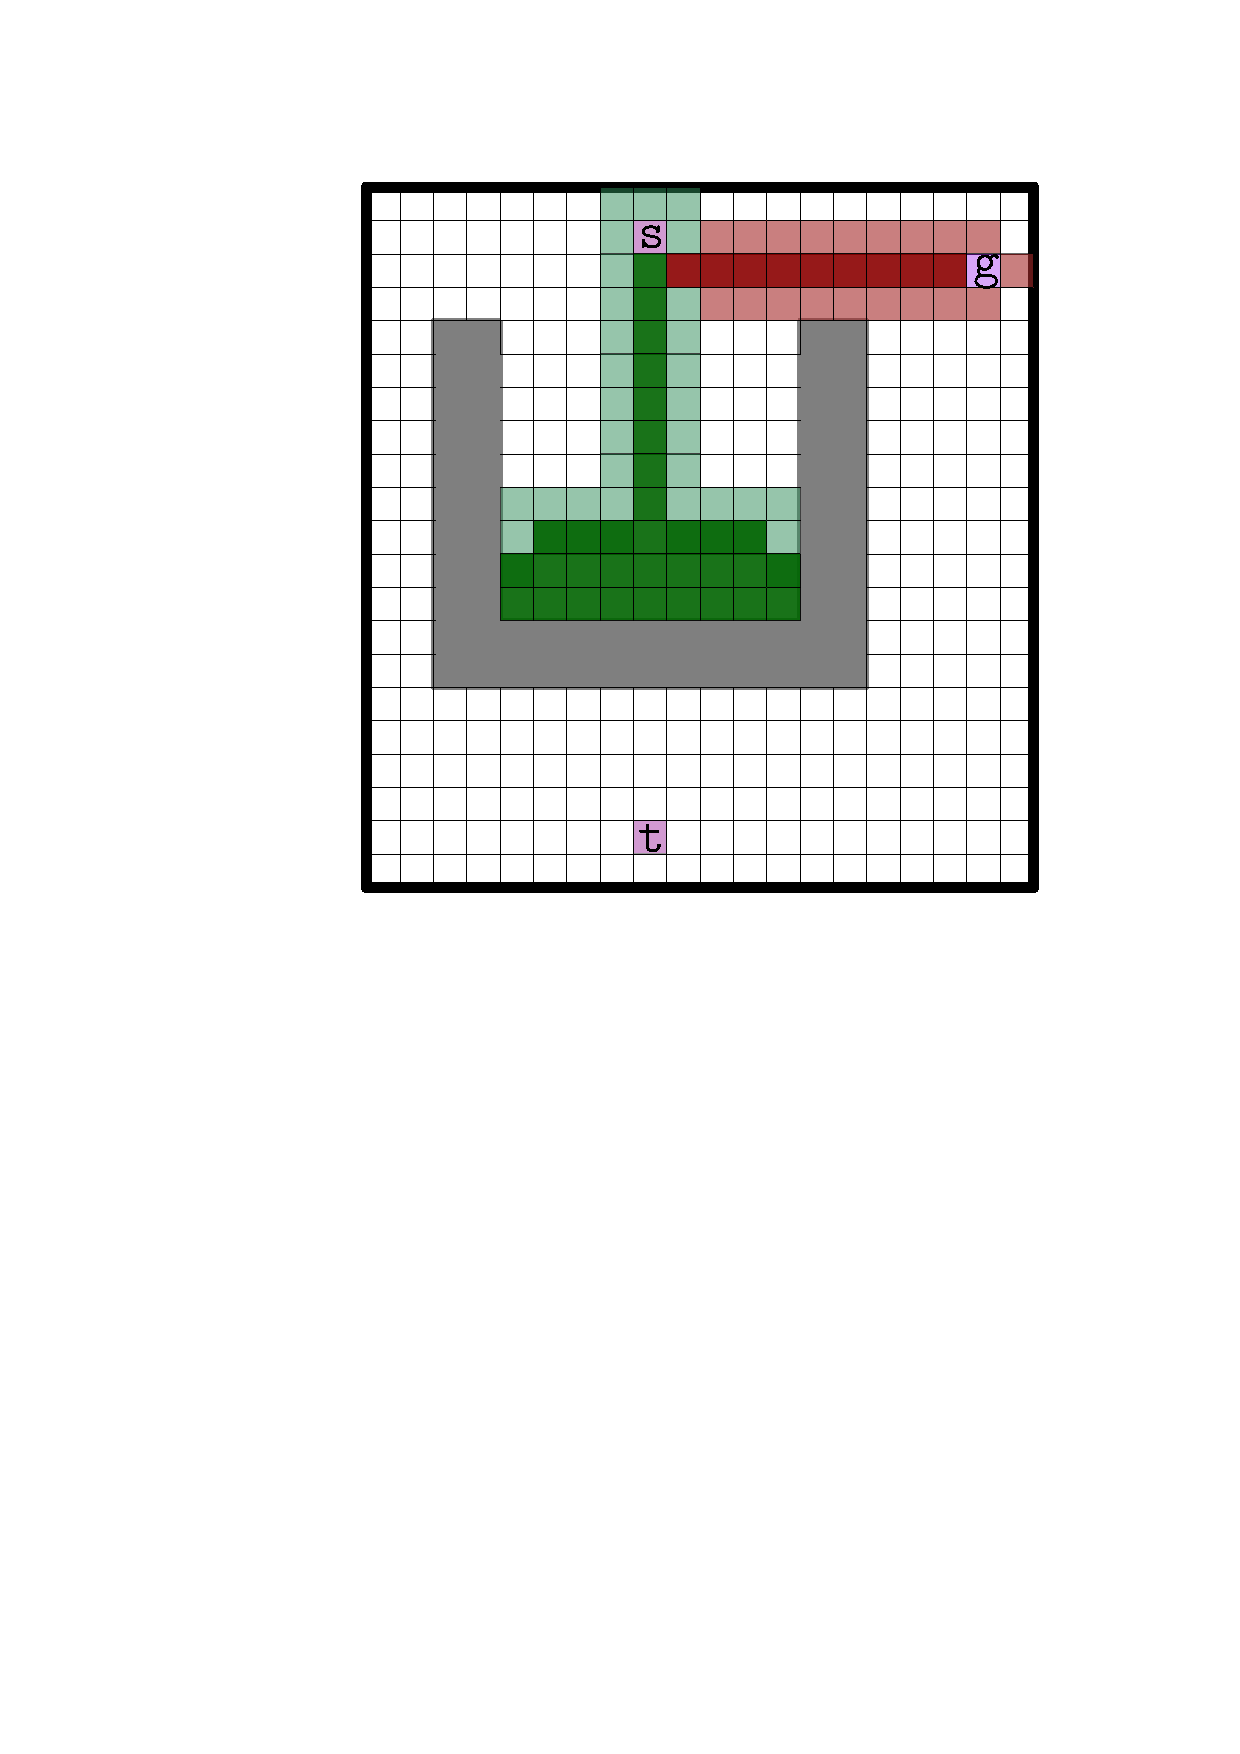
\includegraphics[width=0.225\textwidth]{fig/example_2.pdf}
  }
  \subfigure[]
  {
  \label{fig:dynamic_heuristic3}
  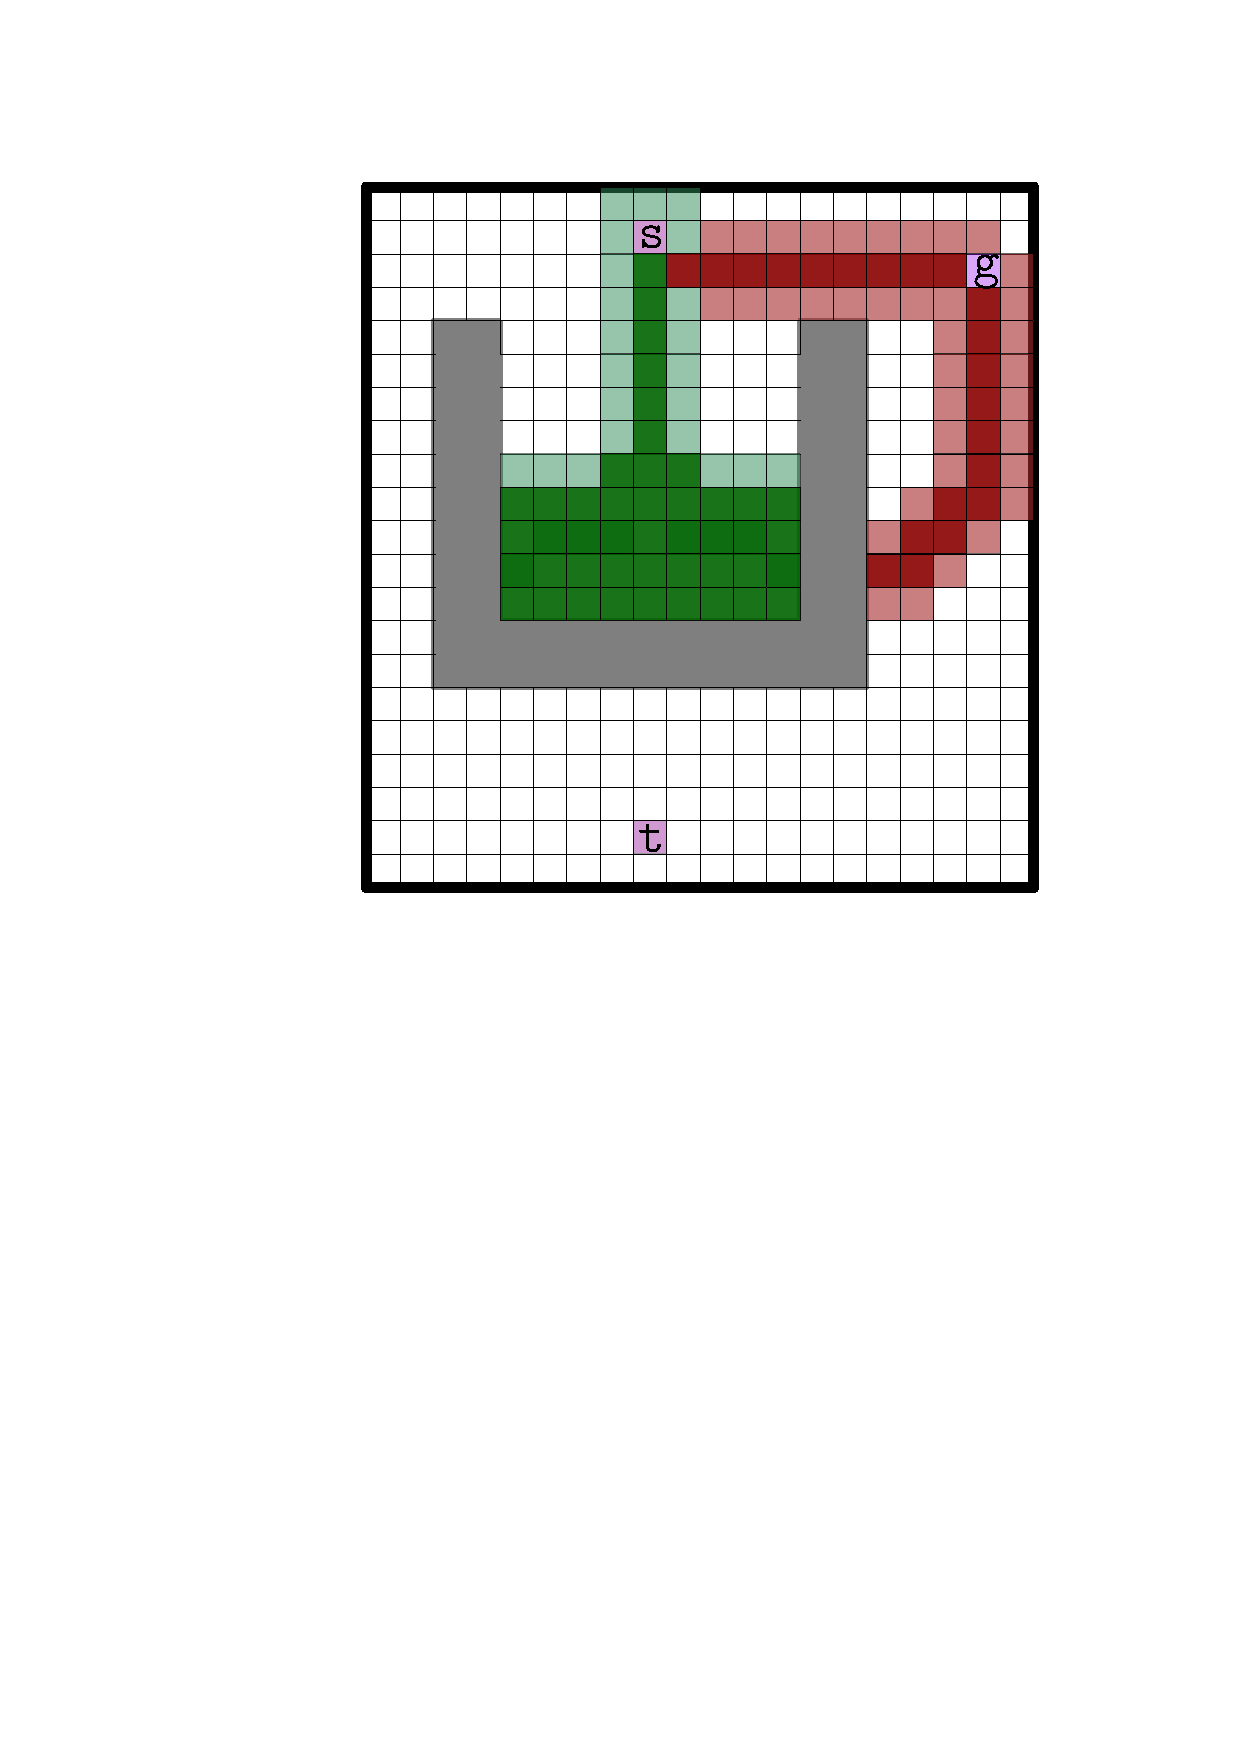
\includegraphics[width=0.225\textwidth]{fig/example_3.pdf}
  }  
  \subfigure[]
  {
  \label{fig:dynamic_heuristic4}
  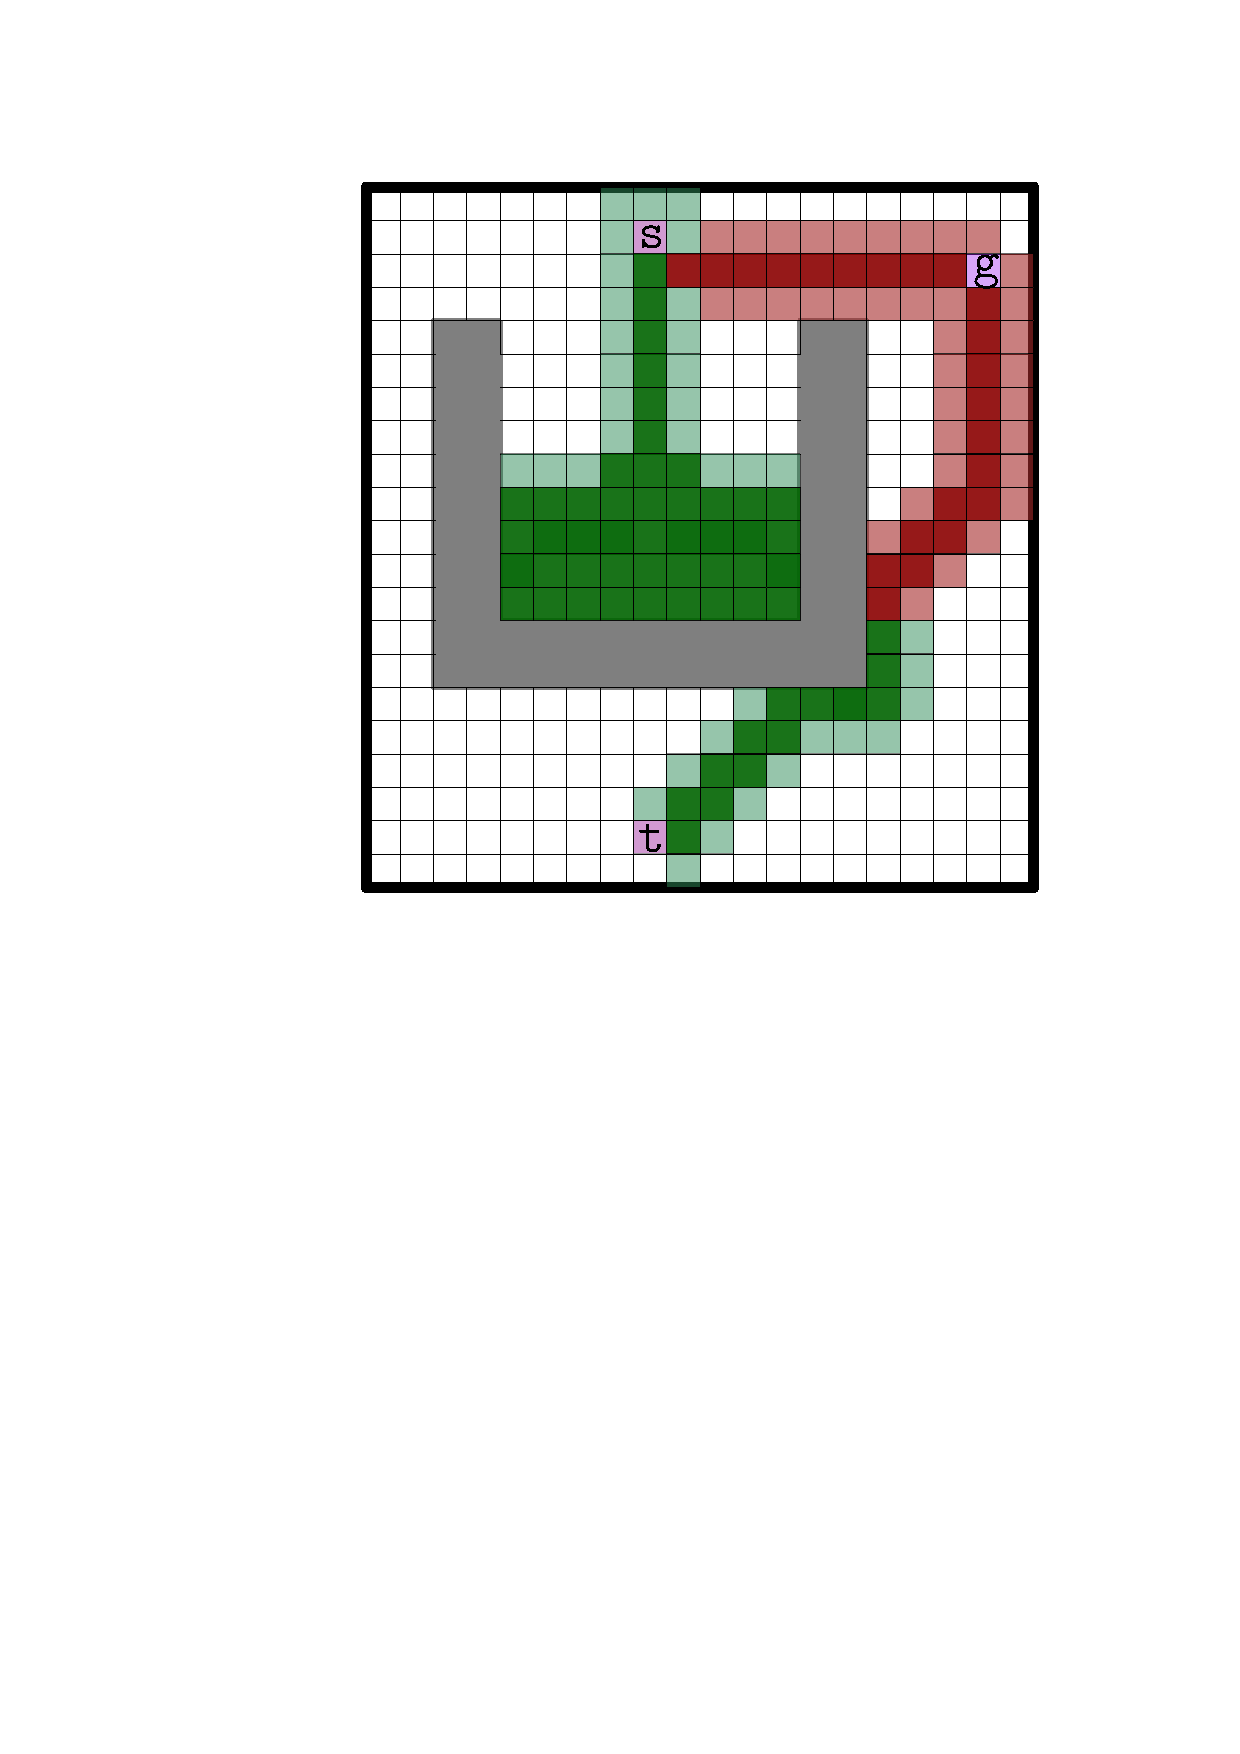
\includegraphics[width=0.225\textwidth]{fig/example_4.pdf}
  }
  \caption{%
    Algorithm progression.
    States popped from a priority queue are depicted using dark colors while states still in a queue are depicted by a light color.
    Start, target and user-guided states are depicted in purple with the letters \texttt{s}, \texttt{t}, \texttt{g}, respectively. 
    %
    In this example MHA* alternates between queues in a round-robin fashion. Furthermore, heuristics are inflated by a weight of $w=\infty$. Namely, the priority queues are ordered according to the heuristic-value of the states.
    %
	\subref{fig:dynamic_heuristic1}~MHA* starts with a single baseline heuristic (green) which is the Euclidean distance to goal and a local minimum is identified.
    %
	\subref{fig:dynamic_heuristic2}~User provides guidance and the algorithm automatically generates an additional heuristic (red) that drives the search towards the guidance (notice that the anchore heuristic continues to search the local minimum).
    %
	\subref{fig:dynamic_heuristic3}~After passing through the guidance, the additional heuristic (red) drives the search towards the goal.
    %
	\subref{fig:dynamic_heuristic4}~After the additional heuristic found states that are placed at the top of the priority queue of the anchor heuristic, the additional heuristic is deleted and the anchor heuristic drives the search towards the goal.
  }%
  \label{fig:filmstrip-dynamic_heuristic}%
  \vspace{-2.5mm}
\end{figure*}



We assume that MHA* has at least one baseline heuristic~$h_{\text{goal}}$ which approximates the cost to reach the goal from every state.
Furthermore, we assume that there exists a family of (possibly inadmissible) heuristic functions $\H$, such that for every configuration~$q$, there exists a heuristic $h_q \in \H$ where~$h_q(s)$ estimates the cost to reach $q$ from state $s$.
%%%%

Given user guidance in the form of a configuration $\hat{q}$, we dynamically generate a new heuristic $$
    \hat{h}(s)= 
\begin{cases}
    h_{\hat{q}}(s) + h_{\text{goal}}(\hat{q}),	& 
    		\text{if } \hat{q} \text{ is not an ancestor of } s,\\
    h_{\textbf{•}{goal}}(s),            		& 
    		\text{if } \hat{q} \text{ is an ancestor of } s.
\end{cases}
$$
Namely,~$\hat{h}$ estimates the 
cost to reach the goal (via the term~$h_{\text{goal}}$) by passing through $\hat{q}$ (via the term $h_{\hat{q}}$). If the state was reached by passing through $\hat{q}$, then the value of $\hat{h}$ is simply the estimation of the cost to reach the goal.


Equipped with the heuristic $\hat{h}$, we add a new queue to the MHA* algorithm prioritized using the heuristic $\hat{h}$. %(Alg~\ref{alg:main}, line~4). 
States expanded using this queue will be biased towards $\hat{q}$ (see also~\cite{INL15} for more details on adding heuristics and queues dynamically to MHA*
and~\cite{NAL15} for more details on dealing with calibrating the different values used by different heuristic functions).
Note that in MHA*, nodes are shared between the different queues.
Thus, once a state has been found that can be used to get the planner out of the \noindent , it will be expanded by the other queues using their heuristics.
Once this is detected 
%(Alg~\ref{alg:main}, line~8),
the newly-added queue is removed.

\subsection{User-guided MHA*}
\label{sec:instantiation}
We are now ready to describe how we apply our general framework of user-guided planning to the case of MHA*.
This differs slightly from the general approach described in Sec.~\ref{sec:high} due to our ability to identify which queue is in a \noindent  and to detect if the configuration~$\hat{q}$ (i.e., the guidance) was reached.

Specifically, if the baseline heuristic escaped a stagnation region but the configuration $\hat{q}$ was \emph{not} reached, we suspend the dynamic queue but do not discard it. 
This is done to avoid querying the user for unnecessary guidance when the previous guidance can still be used.
When the planner will detect that is in a stagnation region, it will first resume the suspended dynamic heuristic (if one exists).

If the baseline heuristic escaped a stagnation region and the configuration~$\hat{q}$ was  reached it can no longer be used and it will be discarded.
Finally, if the dynamic heuristic is in a stagnation region then it is discarded and the user will be queried for a new guidance. 

For pseudo-code describing the algorithm, see Alg.~\ref{alg:instantiation}.
For a visualization of the way the algorithm progresses, see Fig.~\ref{fig:filmstrip-dynamic_heuristic}.
%
%Specifically, the planner can be in a local minima in the dynamically-generated queue that is used to escape the original local minima. 
%In such cases we request new guidance from the user and replace the previous guidance with the new one.


\begin{algorithm}[tb]
\caption{User-guided MHA*}
\label{alg:instantiation}	
\begin{algorithmic}[1]
\small
\While{no solution is found} 
	\While{exists baseline heuristic not in a local minimum}
		\State run MHA*
		\Comment{no user guidance}
	\EndWhile
%	
\vspace{2mm}
%
	\If {exists suspended dynamic heuristic}
		\State {resume using dynamic heuristic}
	\Else
		\State{get user guidance and add dynamic heuristic}		
	\EndIf
%	
\vspace{2mm}
%
	\While{baseline heuristics are in local minima
			\textbf{and} \\
			\hspace{10mm} dynamic heuristic isn't in a local minimum 
	}
		\State run MHA*
		\Comment{use guidance to escape local minimum}
	\EndWhile
%	
\vspace{2mm}
%	
	\If {dynamic heuristic is in local minimum}
		\State {remove dynamic heuristic}
		\Comment{guidance is not useful}
	\Else 	\Comment{dynamic heuristic is not in local minimum}
		\If {states passed through guidance}
			\State {discard dynamic heuristic}
		\Else
			\State {suspend dynamic heuristic}
			\Comment{may be useful in future}
		\EndIf
	\EndIf

\EndWhile
\end{algorithmic}
\end{algorithm}

%%%%%%%%%%%%%%%%%%%%%%%%%%%%%%%%%%%%%%%%%%%%%%%%%%%%%
%Evaluation
%%%%%%%%%%%%%%%%%%%%%%%%%%%%%%%%%%%%%%%%%%%%%%%%%%%%%
\section{Evaluation }
\label{sec:eval}
%We implemented the planning framework described in Sec~\ref{sec:planning} for the case of a humanoid robot. We gave the robot the task of climbing up a set of stairs while avoiding collision with obstacles as well as adhering to the physical constraints of the robot (see Fig.~\ref{fig:robot}).
%We used MHA* with one non-admissible heuristic called the \emph{baseline} heuristic.
%Results demonstrating the effectiveness of our framework are depicted in Fig.~\ref{fig:res}
%as well as in the supplementary video\footnote{
%\url{https://drive.google.com/file/d/0B5cCvECYZLYZYlF2cFFPSmQ1clE/view?ts=591cd6e1}}. 

We evaluated the performance of our planning framework on a 34-DOF WAREC humanoid robot~\cite{MHSetal15} 
which is constrained to maintain static stability at all times by design. The robot has four symmetric limbs having 7 revolute joints each. The other 6 dimensions come from the pose of the robot with respect to some global frame of reference. The initial state of the robot is defined as the full dimensional 34-DOF configuration of the robot whereas the goal state is represented as a cylindrical region which the robot needs to enter (depicted in Fig.~\ref{fig:robot}). As described earlier, our approach runs in the so called tracking phase of the underlying adaptive dimensionality framework, in which the planner attempts to find a plan in the full dimension of the robot in order to track the footstep plan generated in the planning phase. 

\subsection{Implementation details}
We used a set of motion primitives which are short kinematically feasible motion sequences to generate the actions or the successors during the search. The primitives included clockwise and counter-clockwise rotation of individual joints. Three different types of motion primitives are used; 1) primitives for the free limbs of the robot i.e. the limbs whose end effectors are not constrained by any contact surface 2) primitives to move the torso of the robot which requires solving closed chain inverse kinematics for the constrained limbs 3) primitives to latch onto the footstep path which also requires solving inverse kinematics for the target footstep position.

\os{mention that we add a motion primitive to the guidance once we are close to it}

The admissible heuristic which we use as the anchor heuristic in the MHA* search is computed as \os{(discuss with Max)}. On top of that we use only one inadmissible baseline heuristic which assists the search with a general walking or stepping capability for the robot but is not intelligent enough to encounter contingencies e.g an obstacle in the way or if the robot needs to make use of a support surface in order to make further progress towards the goal. Again the idea here is to have a small number of reasonably generic baseline heuristics and eliminate the need to hand engineer several domain specific heuristics. The dynamic heuristic that we used is the euclidean distance in the joint 34-DOF space.

\subsection{Climbing a staircase}
\os{should we have the simple case (RSS version?)}

We gave the robot the task of climbing up a set of stairs while avoiding collision with obstacles (steps and handrails) as well as adhering to the physical constraints of the robot (see Fig.~\ref{fig:robot}). In the absence of handrails the planner successfully finds a path to the goal without invoking the user for guidance. The handrails make the planning problem  harder. As the robot has to sway sideways during the stepping motion to maintain static stability, the handrails make it harder for the robot to climb up the staircase if it make use of them for support. To this end we allow the user to provide guidance to the planner to be able to use support surfaces. We pre-specify a set of valid contact surfaces (handrail cylinders in this experiment). When the user brings any of the robot hands within a threshold distance to a valid contact pose on a support surface, the GUI snaps the robot state to establish a valid support contact by solving the inverse kinematics for the respective limb. The planner incorporates this contact information in the robot stability calculations. Resultantly when the user provides such a guidance, the dynamic heuristic guides the search to reach this user provide state and continues to expand its successor states with the hand contact because they enable the search to make further progress. In the context of motion primitives, in this case we allow two types of motions for the robot torso, one with the hands in contact and the other that allow free motions for the robot arms. This helps the robot to let go of the handrail when it no longer needs the support.

Results demonstrating the effectiveness of our framework are depicted in Fig.~\ref{fig:res}
as well as in the supplementary video\footnote{
%\url{https://drive.google.com/file/d/0B5cCvECYZLYZYlF2cFFPSmQ1clE/view?ts=591cd6e1}}. 
\os{ADD LINK TO VIDEO}}
\begin{figure}[tb]
  \centering
  	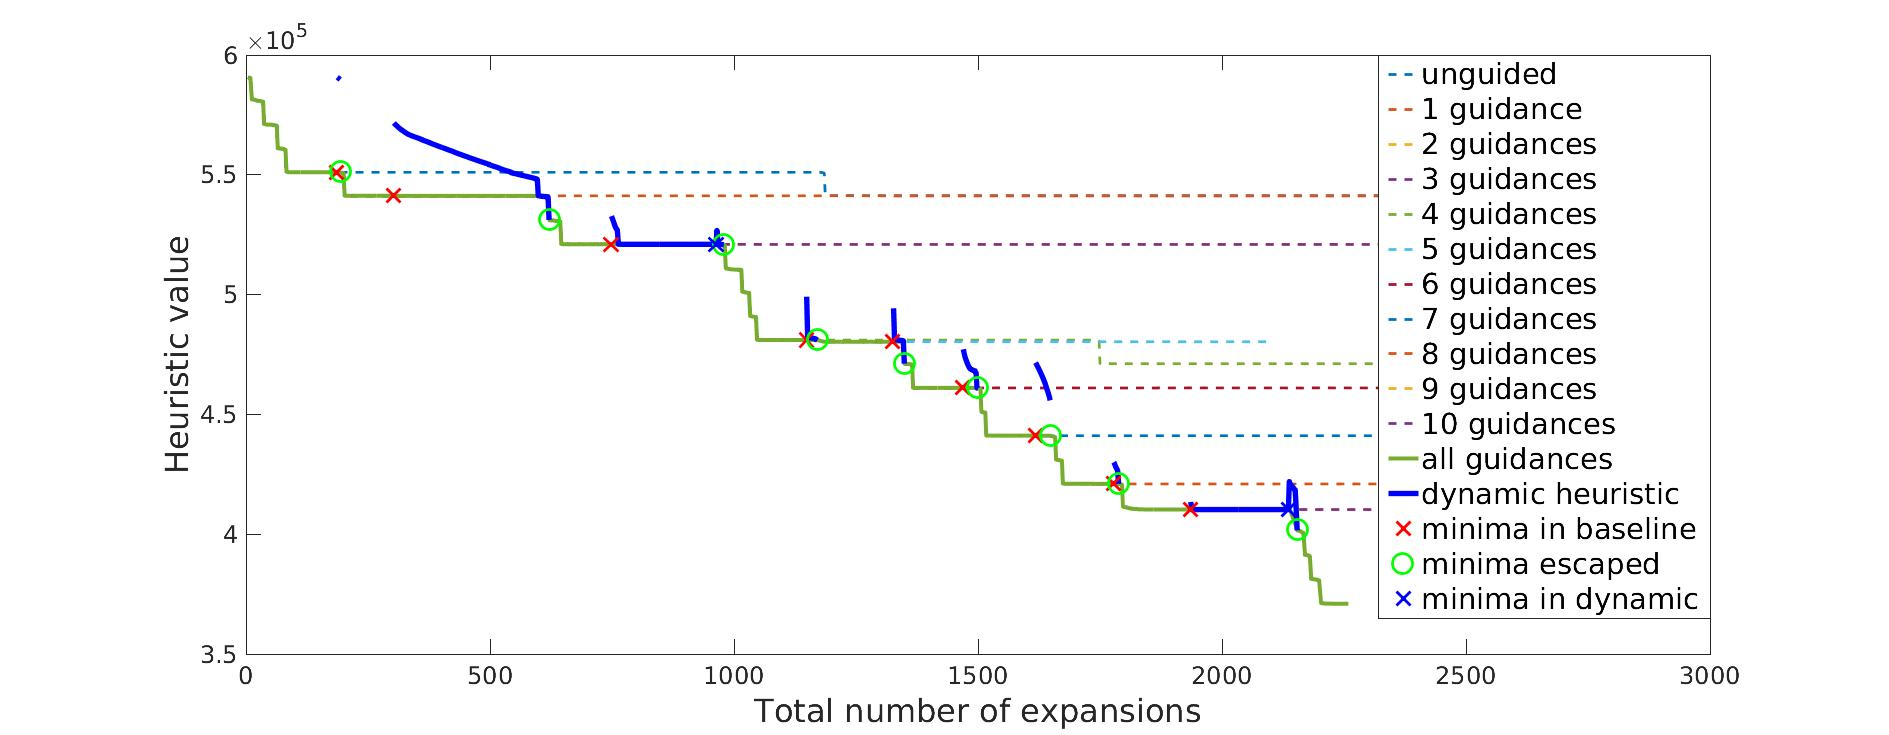
\includegraphics[width=0.49\textwidth, trim={5cm 0 5cm 0},clip]{fig/h_staircase.jpg}
  	\vspace{-2mm}
  \caption{
		Progress of MHA* with and without user guidance---heuristic values as a function of the number of queue expansions.
		When a local minima is detected (red cross) in the baseline heuristic (cyan), a dynamic heuristic is generated (blue) until the local minima is escaped (green circle) or until a new local minima is detected (blue cross) in the dynamic heuristic.
		Plots depicting the baseline heuristic values when only a limited amount of guidance is given demonstrate that without guidance, the planner remains stuck in local minima (we note that as MHA* is complete, it will eventually escape all local minima).
		}
\vspace{-5mm}
   	\label{fig:res}
\end{figure}

\subsection{Crawling to ladder climbing}


\subsection{Robustness to algorithmic parameters}
%%%%%%%%%%%%%%%%%%%%%%%%%%%%%%%%%%%%%%%%%%%%%%%%%%%%%
%Discussion and future work
%%%%%%%%%%%%%%%%%%%%%%%%%%%%%%%%%%%%%%%%%%%%%%%%%%%%%
\section{Discussion and future work}
\label{sec:future}

\subsection{Discussion}
In Sec.~\ref{sec:eval} we demonstrated how using user guidance allows to solve highly-constrained motion-planning in high-dimensional spaces with only simple baseline heuristics.
An alternative approach would be to add domain-dependant carefully-crafted heuristics~\cite{V17} which allow to faster solve the same problems completely autonomously.
\os{Add citation to alternative submission if arXiv version exists}


When a new type of problem is encountered 
(say, climbing a ladder, crawling on uneven terrain etc.)
we can either design additional heuristics to tackle this problem or shift the burden to the user to provide guidance in an online fashion.
If our problem requires planning in multiple, diverse types of domains this problem is accentuated---should we  use a large arsenal of heuristics that can address each domain or should we have a small number of baseline heuristics that will (roughly) address all domains and rely on user guidance when these baseline heuristics fail?
Clearly, there is no clear answer to this question and our approach simply offers a general alternative to existing approaches.


\subsection{Future work}
While providing promising initial results, our framework is far from being complete.
We are interested in experimenting with alternative forms of user guidance such as providing a \emph{constrained sub-manifold} of the configuration space. This may be used to guide the humanoid to use the railing while planning the stairs.
%Furthermore, we would like to have a \emph{recursive} implementation of our framework.
%Namely, the planner can be in a local minima while trying to escape a local minima. This should be identified and then the user should either (i)~provide new guidance 
%\os{This is already implemented}
%or 
%(ii)~provide  guidance  toward the previoulsy provided guidance.
Finally, once a guide is given, we want our planner to be able to \emph{generalize} the guidance obtained to future local minima that are similar in nature to the ones encountered.

\os{add discussion on implementation of approach in the context of sampling-based planners}

%\newpage

%\bibliographystyle{plainnat}
\bibliographystyle{abbrv}
\bibliography{bibliography}

\end{document}

%%% Local Variables:
%%% mode: latex
%%% TeX-master: t
%%% End:
